\documentclass[12pt]{article}
\usepackage{graphicx}

\title{COP290: User Registration App}
\author{User1 (Entry number 1) \\ User2 (Entry number 2) \\ User3 (Entry number 3) }

\begin{document}
\maketitle

Mention the detailed description of what the application does.

\section{User Interface}

\begin{figure}[!ht]
	\centering
	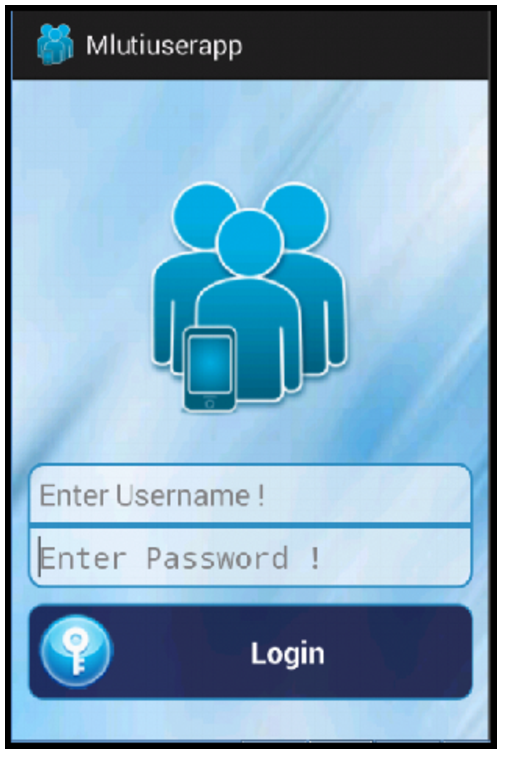
\includegraphics[width=0.5\textwidth]{./UserInterface}
	\caption{Primary Screen}
\end{figure}

\begin{itemize}
\item Details of the screens visible to the user
\item Animations, buttons (enabled/disabled under what conditions)
\item Actions performed when a user enters information, presses a button/icon etc.
\end{itemize}

\section{Implementation Details}

\begin{itemize}
\item Organization of user information (Is it in a special User class, or is it distributed in arrays for each user entry)
\item Methods to verify the user information: Highlight the errors handled by the code
	\begin{itemize}
		\item How to make sure that the user is entering a valid entry number
		\item How to make sure that the user is entering a valid name
	\end{itemize}
\item Methods for network communication. You can cite material that you used to create the application~\cite{android_network_tutorial}.
\end{itemize}

The code for the project is being maintained in this repository: {\em https://prathmesh\_kallurkar@bitbucket.org/prathmesh\_kallurkar/user-registration-app.git}.

\bibliographystyle{abbrv}
\bibliography{references}

\end{document}
